\documentclass{beamer}
\usepackage{beamerthemesplit}
\usepackage{graphicx,url}
\usepackage[brazil]{babel}
\usepackage[utf8]{inputenc}
\usepackage{multimedia}

\mode<presentation>
{
  \usetheme{Ilmenau}
  \setbeamercovered{transparent}
}

\newcommand{\eng}[1]{\textit{#1}}
\newcommand{\obra}{\textit{Em torno da romã}}
\newcommand{\goiaba}{\textit{Goiaba}}
\newcommand{\redmark}[1]{\textcolor{red}{#1}}
\newcommand{\graymark}[1]{\textcolor{gray}{#1}}
\newcommand{\tocar}{\textcolor{blue}{$\blacktriangleright$}}

\title{Functional Harmonic Analysis and Computational Musicology in
  Rameau}

\author{Alexandre Tachard Passos, Marcos Sampaio, Pedro Kröger,
  Givaldo de Cidra}
\date{7 de setembro de 2009}

\logo{
\includegraphics[scale=.15]{logo-genos}}

\begin{document}

\frame{\titlepage}

\frame{
  \frametitle{O que é o Rameau}
  \begin{itemize}
  \item Um framework pra implementar algoritmos musicológicos e
    algoritmos de análise harmônica
  \item Um programa com vários desses algoritmos já implementados
  \end{itemize}
}

\frame{
  \frametitle{Algoritmos musicológicos}
  \begin{itemize}
  \item Oitavas e quintas consecutivas
  \item Cruzamento de vozes
  \item Diferença para âmbito de vozes de Kostka e Payne
  \item Saltos melódicos
  \item Resolução de sétimas
  \item Progressões strong, weak, superstrong e neutral (Schoenberg)
  \item Cadências
  \end{itemize}
}

\begin{frame}
  \frametitle{Exemplo musicológico: Incidência de tipos de cadências}
  \texttt{\$ rameau cadences --cloud -f chor:130}
  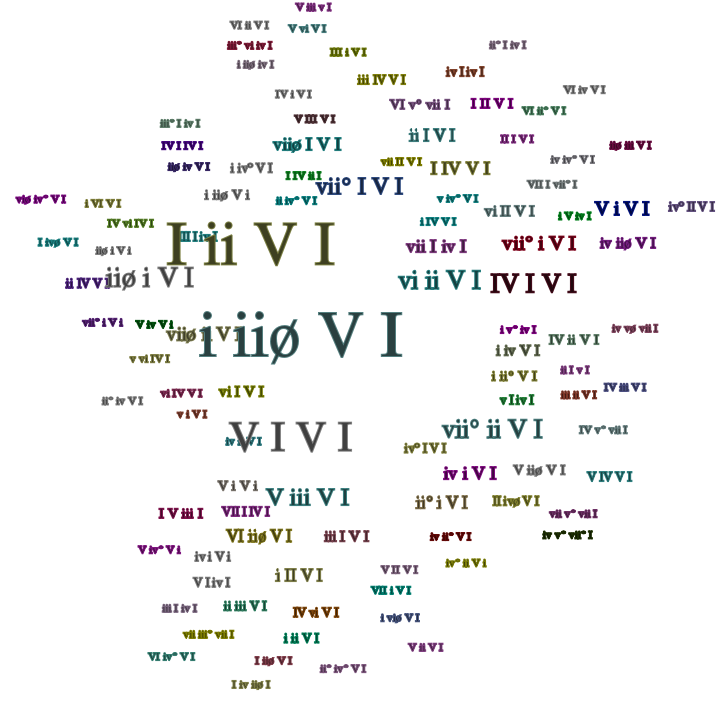
\includegraphics[scale=.35]{cadences}
\end{frame}

\frame{
  \frametitle{Exemplo análise funcional}

  \texttt{\$ rameau functional -S -f chor:130}
  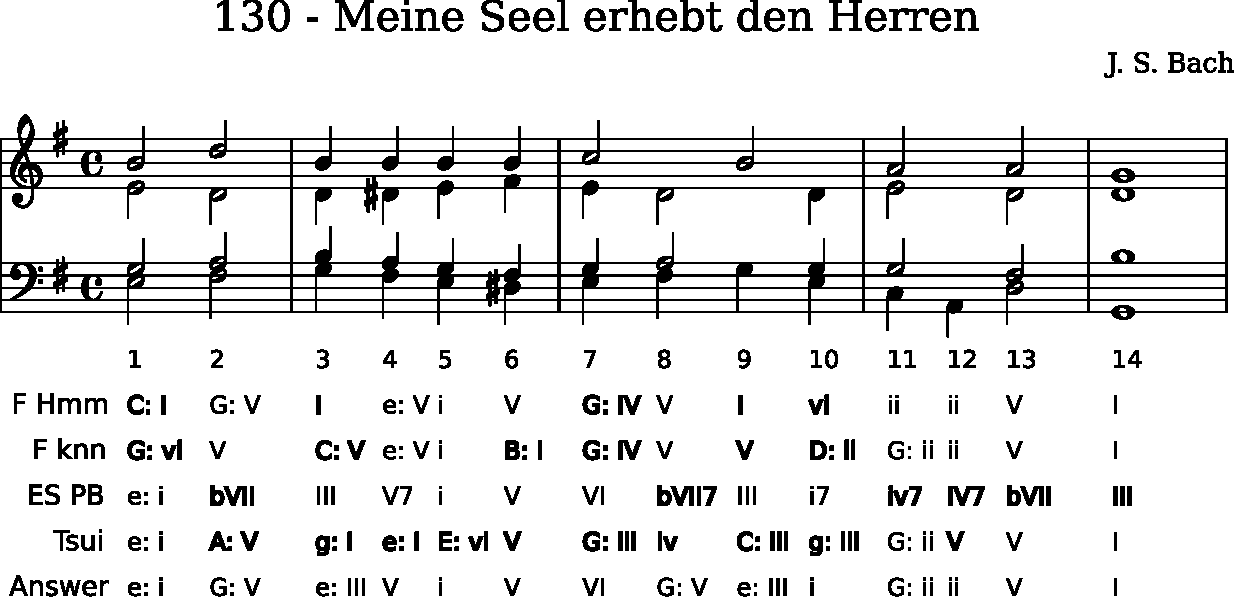
\includegraphics[scale=.45]{analysis-functional-130}
}

\frame{
  \frametitle{Exemplo identificação de acordes}

  \texttt{\$ rameau analysis -S -f chor:130}
  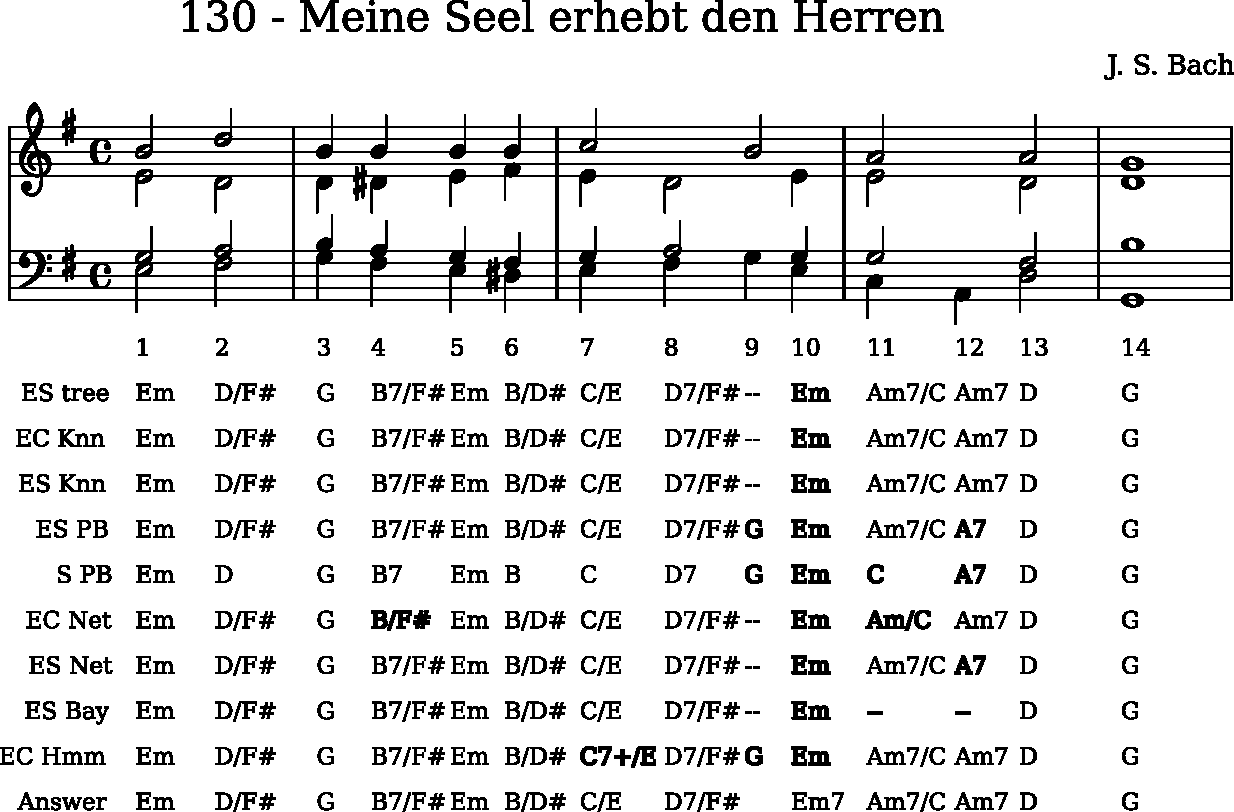
\includegraphics[scale=.45]{analysis-130}
}

\frame{
  \frametitle{Interface web}

  \texttt{\$ rameau web}

  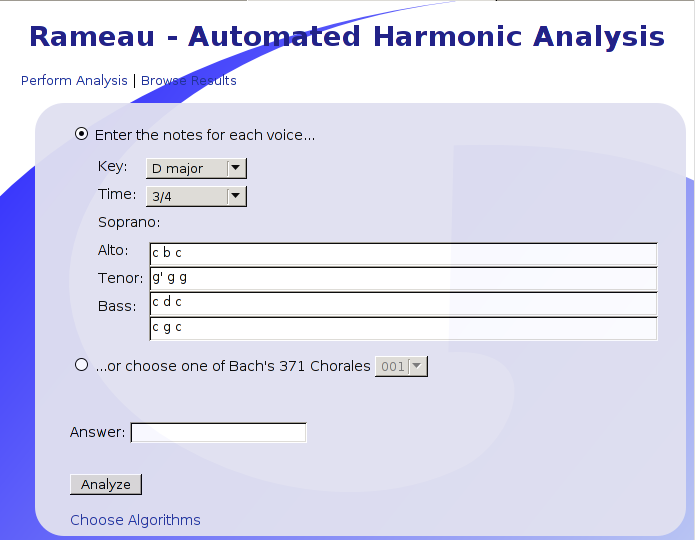
\includegraphics[scale=.33]{rameau-web}
}

\frame{
  \frametitle{Conclusões e trabalhos futuros}
  \begin{itemize}
  \item Software mais maduro
  \item Implementações para várias funções musicológicas
  \item Implementação de 9 algoritmos
  \item Arquitetura ainda limitada a textura a 4 vozes
  \end{itemize}

  Futuro: Corpus Humdrum/Kern

  \tiny
  Disponível em \url{http://genos.mus.br/rameau}
}

\end{document}
